%%%%%%%%%%%%%%%%%%%%%%%%%%%%%%%%%%%%%%
%%  
%% Chapter 5: Memory Movement
%%
%%%%%%%%%%%%%%%%%%%%%%%%%%%%%%%%%%%%%%

\def\ArtDir{05.MemMove/figures}%

\chapter{Memory movement}
\label{chapter:memory}

\section{Recap implicit data movement}
\begin{itemize}
  \item So far only could work with scalars and stack arrays.
  \item Now we explain heap arrays.
  \item Recall firstprivate clause.
  \item The pointer itself will be mapped firstprivate.
  \item But the data needs to be mapped\dots
\end{itemize}

\section{Explicit data sharing with the map clause}
\subsection{Array syntax: important as non-intuitive in C}
\begin{itemize}
  \item Introduce OpenMP array notation.
  \item array[start:length].
  \item It is not array[start:end] in C.
  \item Follows pointer size rules, so don't have to worry about sizeof(T).
  \item Array notation in Fortran.
\end{itemize}

\subsection{The map clause}
\label{ssec:map_clause}
\begin{itemize}
  \item Map clause on a target directive.
  \item List notation of things to map.
  \item to, from and tofrom.
  \item Recall the scoped behaviour: from transfer happens on the closing curly brace.
  \item alloc and delete and release.
  \item Pointer attachment from OpenMP 5.0
  \item Some mention of reference counting. Things only transfer based on that. Read the spec for the details.
\end{itemize}

\subsection{Example: Vector add on the heap}
\begin{itemize}
  \item Similar to vector add example so far.
  \item Arrays now allocated on the heap.
  \item Show use of map(tofrom) clauses to copy the data to the device, run in parallel, then copy back at end.
\end{itemize}

\section{Reductions and mapping back result.}
\label{sec:target_reductions}
\begin{itemize}
  \item In OpenMP 5, the reduction result is brought back automatically.
  \item Need to add a note that in OpenMP 4.5, need to use the map clause to do a reduction on the device.
  \item map(tofrom: scalar)
  \item Explain that without this it is firstprivate and not copied back.
  \item Explain interaction of reduction clause with teams and threads and simd in the OpenMP hierarchy of parallelism.
\end{itemize}

\subsection{Example: Pi}
\begin{itemize}
  \item Show pi reduction example.
  \item Has no data arrays to map.
  \item But need to map the reduction result.
\end{itemize}

\section{Data regions}
\begin{itemize}
  \item Motivation: so far expressed data movement for each target region.
  \item Wasteful as can often just leave it there between target regions.
  \item Multiple target regions, leaving data resident.
  \item Motivating example: multiple subsequent transformations to data, and/or iterative solve.
  \item Wasteful as only want to do the mapping: both writing and in terms of optimal data movement.
  \item Idea of target data region. Inherited by target regions. Data already exists on the device.
\end{itemize}

\subsection{Target data directive}
\label{ssec:target_data}
\begin{itemize}
  \item Scoped target data region.
  \item Useful for lots of kernels running after each other.
  \item Show an example of this.
  \item No need to map on the target regions themselves.
  \item Downsides are the structured block requirements.
  \item From destination determined at start of region.
\end{itemize}

\subsection{Target enter/exit data}
\label{ssec:target_enter_exit_data}
\begin{itemize}
  \item Change target data environment in unstructured way.
  \item Expect will need to talk about reference counting again.
  \item Useful because don't need scoped. But behaves similarly.
  \item Example use just after every allocation.
  \item Means this helps with C++ class data in constructors.
  \item Example: Show the same target data example with the target enter/exit data.
\end{itemize}

\subsection{Target update directive}
\label{ssec:target_update}
\begin{itemize}
  \item Need to get data back in the middle of target data region.
  \item target update directive.
  \item Uses same map clauses as before.
  \item Example: convergence, or halo exchange.
\end{itemize}

\subsection{Pointer swapping}
\begin{itemize}
  \item Pointers are mapped firstprivate and zero-length arrays.
  \item Updates reference count.
  \item Doesn't need to copy any data, and don't need to specify length as already mapped.
  \item Will be remapped/reevaluated on each target region.
  \item How do you do pointer swapping in a target data region.
  \item How do you do pointer swapping when you use target enter/exit.
\end{itemize}

\section{Example: Jacobi or CG or simple linear solver.}
\begin{itemize}
  \item Biggest example, showing off everything so far.
  \item Key requirements: iterative and pointer swap to motivate cutting down memory movement
  \item Use target enter/exit data regions.
  \item Use pointer swapping.
  \item Use target update.
  \item Uses parallelism, with/without reduction clause.
\end{itemize}

\section{Unified shared memory}
\label{sec:usm}
\begin{itemize}
  \item OpenMP 5 add requires directive
  \item Which unified shared memory is.
  \item Data moves back and from at will (page fault).
  \item Requires hardware support.
  \item Pros: each to get started, as don't have to map.
  \item Cons: parallelism is the easy bit, it's the data movement which is important.
  \item In 5.0, limited performance tuning opportunities.
  \item Mapping gives you the control for optimal performance.
\end{itemize}


\section{Advanced parts}
\subsection{Declare target}
\label{ssec:declare_target}
\begin{itemize}
  \item map global variables
\end{itemize}


\subsection{User-defined mappers}
\label{sec:mapper}
\begin{itemize}
  \item From OpenMP 5.0
  \item Allow user to define how structures are mapped.
  \item Useful for complex structures
  \item Example: struct with a pointer variable. Declare mapper of struct which also maps the pointer.
\end{itemize}

\subsection{Allocator and memcpy APIs and related clauses}
\label{sec:alloc_apis}
\begin{itemize}
  \item \Code{omp\_target\_alloc()}
  \item \Code{omp\_target\_free()}
  \item \Code{use\_device\_ptr}
  \item allocate, test, and move memory using the APIs instead of the pragmas.
\end{itemize}


%-----------------------------------------------------------------------
%------------------------- From Next Step ------------------------------
%-----------------------------------------------------------------------
\section{From The Next Step Chapter 6}
\subsection{Heterogeneous Memory Model}
\label{ssec:06.heterogeneous-memory-model}

\index{Accelerators!Device constructs}
%Code executing on a device is typically not very useful without some data to
%compute on.  
This section provides an overview of the \OMP\ heterogeneous memory model.
The device constructs, clauses, and runtime functions that control how data is shared
between threads executing on the host and an accelerator device are listed below:

\begin{itemize}
  \item Map and Defaultmap Clauses
  \item Target Data Construct
  \item Target Enter and Exit Data Constructs
  \item Target Update Construct
  \item Declare Target Directive
  \item Use\_device\_ptr and Is\_device\_ptr Clauses
  \item Device Memory Functions
%  \item Runtime Functions
%  \begin{itemize}
%    \item \code{omp_target_alloc}
%    \item \code{omp_target_free}
%    \item \code{omp_target_is_present}
%    \item \code{omp_target_memcpy}
%    \item \code{omp_target_memcpy_rect}
%    \item \code{omp_target_associate_ptr}
%    \item \code{omp_target_disassociate_ptr} 
%  \end{itemize}
\end{itemize}

\index{OpenMP clauses!map}
\index{Accelerators!Map clause}
Of these, by far the most important is the \code{map} clause.  Recall from
Chapter~\ref{chap:recap} that variables are shared or private.  As of \OMPfourzero,
variables can also be \emph{mapped}, which is the concept that \OMP\ uses to
describe how data is shared across devices.  The \code{defaultmap} clause can
change the default rules for determining if certain variables are either
private or mapped.  The general concepts of mapped variables
are discussed later in this section.  
The syntax and mechanics of the \code{map} and \code{defaultmap} clauses
are covered in Section~\ref{sec:06.data-mapping-clauses}.

The host and accelerator may have different representations for the address of
a variable.  The \code{use_device_ptr} and \code{is_device_ptr} clauses are
provided for the instances in which this difference in address representation
must be dealt with explicitly.  These device pointer clauses are covered in
Section~\ref{sec:06.Device-pointer-clauses}.

Variable's with static storage (for example, global variables) may be mapped
for the entire program using the \code{declare target} directive, which is
covered in Section~\ref{sec:06.declare-target-construct}.

The \code{target}~\code{data}, \code{target}~\code{enter}~\code{data},
\code{target}~\code{exit}~\code{data}, and \code{target}~\code{update}
constructs are used to reduce the performance overhead of copying data between
the host and an accelerator.  These data-mapping constructs are
covered in Section~\ref{sec:06.data_mapping_constructs}.

The device memory functions are described in detail in
Section~\ref{ssec:02.new_runtime_functions_3} starting on
page~\pageref{ssec:02.new_runtime_functions_3}.  
The \code{omp_target_is_present} function determines if a variable
is mapped.  Otherwise, the other device memory functions 
manage dynamically allocated device memory.  
Section~\ref{sec:06.device-memory-routines} has examples 
that demonstrate how to use these functions.
%These low-level functions are
%essential for more advanced operations.

%-----------------------------------------------------------------------
%------------------------- New subsection ------------------------------
%-----------------------------------------------------------------------
\subsection{Mapped Variables}
\label{ssec:06.mapped-variables}
\index{Mapped variable}

\index{Accelerators!Initial thread}
Threads executing on an accelerator can have private variables.  The initial
thread that begins the execution of a target region gets a private instance of
a variable that appears in a \code{private} or \code{firstprivate} clause on the
\code{target} construct.  For a \code{firstprivate} clause, the private variable
is initialized with the value of the original variable from the host thread
that encountered the construct.  Likewise, any automatic (stack)
variables that are declared in a scope contained within the construct
are private to the initial thread.

%How do the host and accelerator threads share variables?  
\OMP\ threads 
share variables that are stored in a single shared memory.  However, 
heterogeneous architectures do not always have memory that is symmetrically shared between
host and accelerator devices.  A very common example of a 
heterogeneous architecture like this is one where the accelerator is a card 
and communication to the accelerator occurs over a PCIE bus. 

As shown in figure~\ref{figure:chapter-6-device-memory-types}, \OMP\ supports
heterogeneous architectures with both distributed and shared memory by \emph{mapping}
variables from the host to an accelerator.
When the host and accelerator device do not share memory, a mapped variable
is copied from the host's memory into the accelerator's local memory.
Mapping hides whether or not a variable is shared by or copied to a device.
Based on a heterogeneous architecture's memory system, the \OMP\
implementation does what is required, either sharing or copying a variable when it
is mapped.

\begin{figure*}[!tbhp]
\centering
\pdfimageresolution 400
\fbox{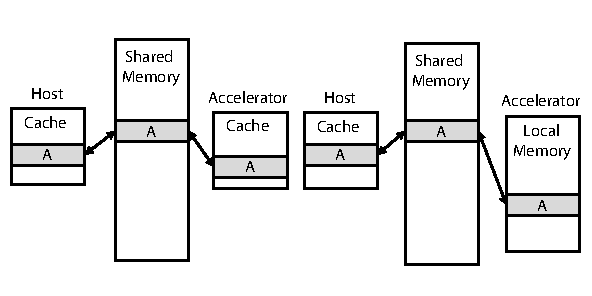
\includegraphics[clip=true,scale=1.00]
         {\ArtDir/device-memory-types.pdf}
     }
\caption{ \textbf{A mapped variable in shared or distributed memory} -- \small
        A mapped variable may be in either shared or distributed memory.
        The OpenMP implementation determines if copies are required.
        }
\label{figure:chapter-6-device-memory-types}
\end{figure*}

\index{Memory consistency!Model} 
How does one ensure that threads on different devices see the same
value of a mapped variable and when?  For the most part, the \OMP\ memory
consistency model as outlined in Chapter~\ref{ssec:01.memory_model}, starting on
page~\pageref{ssec:01.memory_model}, is extended to mapped variables.  

A mapped variable is similar to a shared variable.  Without some 
type of synchronization, two threads executing on
different devices cannot simultaneously access the same mapped variable if
either of the threads writes to the variable.  

\index{OpenMP clauses!map}
\index{Accelerators!Map clause}
Threads executing on different devices may see a consistent value of a mapped
variable at points that are determined by the effects of the \code{map} clause
and the \code{target update} construct.

If memory is distributed, then mapping a variable requires memory allocation,
copy, and flush operations.  The allocation and copy operations are not
required (or are trivial) when memory is shared, but the flush
operation is still necessary.  Although the underlying machinations of variable mapping
is handled by the \OMP\ implementation, it is important to be aware
of the dual-nature of mapped variables to write programs that 
achieve good performance across different architectures.  

%Because the instances of a mapped variable may be in different address spaces,
Because two devices may not share the same address space,
the address of a mapped variable may not be the same on two devices
When a pointer variable is mapped, only the pointer is synchronized, not the
block of memory it points to.  However, array sections may be used to map the
pointed-to memory.

%\index{OpenMP clauses!map}
%\index{Accelerators!Map clause}
%Variables are explicitly mapped using the \code{map} clause (see
%Section~\ref{sec:06.map-clause}).  For variables referenced in a \code{target}
%construct that do not appear in a \code{map}, \code{private},
%\code{firstprivate} or \code{is_device_ptr} clause, data-mapping rules
%determine if they are mapped or private (see
%Section~\ref{ssec:06.defaultmap-clause}).

%Since there might be two copies of the variable, there is a policy for
%maintaining the consistency of the different copies of the variable.
%For example, if a thread on the accelerator writes to a mapped variable, when
%can a thread on the host device see the updated value of the variable?  

%-----------------------------------------------------------------------
%------------------------- New subsection ------------------------------
%-----------------------------------------------------------------------
\subsection{Device Data Environments}
\label{ssec:06.device-data-environments}

\index{Accelerators!Device data environment}
\index{Device data environment}
An accelerator has a \emph{device data environment} that contains the set of
all variables currently accessible by threads running on that device.  As we
discussed in the previous section, host threads share variables with target
device threads by mapping them.  Mapping a variable ensures that the variable
is in the data environment of an accelerator.

\index{Device data environment!Orginal variable}
\index{Device data environment!Corresponding variable}
An \emph{original} variable in a host thread's data environment is mapped to a
\emph{corresponding} variable in the accelerator's data environment.
Depending on the availability of shared memory between the host and target
devices, the original and corresponding variables are either the same variable
allocated in shared memory, or they are allocated in different memories and
copy operations are required to keep the original and corresponding variables
consistent. Whether a mapped variable uses shared or distributed memory is 
taken care of by the \OMP\ implementation.

\index{Device data environment!Present in}
There only can be one instance of a variable in a device data environment.  The
\OMP\ implementation keeps track of which variables are mapped.  If a variable
is already \emph{present} in a device data environment, mapping it again will
find the variable is already there and increment a reference count.  It
will not allocate another instance of the variable.

Minimizing the transfer of data between the host and an accelerator is often
critical to getting good performance on heterogeneous architectures.
Repetitively mapping a variable that is reused by multiple \code{target}
constructs is potentially inefficient.  The \code{target}~\code{data},
\code{target enter data} and \code{target}~\code{exit}~\code{data} constructs amortize data
transfers by mapping variables across the execution of multiple \code{target}
constructs.  Further, the \code{declare}~\code{target} construct can map static and
global variables for the whole program.  Once a variable is mapped to an
accelerator, situations can arise where the value of the variable must be
updated from or to the device, and the \code{target}~\code{update}
construct fulfills this need.  The \code{omp_target_is_present} runtime
function is used to test if a variable is mapped.  
\index{Accelerators!omp\_target\_is\_present} 
\index{OpenMP runtime functions!omp\_target\_is\_present} 

%-----------------------------------------------------------------------
%------------------------- New subsection ------------------------------
%-----------------------------------------------------------------------
\subsection{Device Pointers}
\label{ssec:06.device-pointers}

\index{Accelerators!Device constructs}
Because shared and distributed memory is supported, the \OMP\ memory model
assumes that the host and accelerator data environments are in different
address spaces.  However, this assumption creates some restrictions on
accessing the address of the variable.
% Ruud - I hope this change is OK
% A programmer using the \OMP\ device constructs must be aware of the different
With the \OMP\ device constructs, the user must be aware of the different
address spaces and be careful when using pointers.  
If the host and accelerator do not share memory, their local memories are in
different address spaces.  When a variable is mapped to an accelerator's data
environment, a copy occurs, and the address of the variable on the accelerator
is not the same as the address of the variable on the host.

Memory addresses are stored in pointer variables.  A host thread cannot access
memory via a pointer variable that contains an accelerator address.  Likewise,
an accelerator thread cannot access memory via a pointer variable that contains
a host address.  
Further, the host and accelerator may have different representations for the
address of a variable.  For example, the value of a memory address might
require 64 bits on a host and 32 bits on an accelerator.

In Figure~\ref{figure:chapter6-devptr1}, the host pointer variable \code{hptr} is
assigned the address of a memory location in the host's address space.  
Mapping \code{hptr} copies the value of the pointer variable to the accelerator. The
access to \code{hptr} at line $6$ in the target region by an accelerator thread is illegal.
The accelerator thread is attempting to access a host address.

Likewise in Figure~\ref{figure:chapter6-devptr2}, the accelerator pointer
variable \code{dptr} is assigned the address of a memory location in the
accelerator's address space.  The access to \code{dptr} at line $7$ by a host thread is illegal.

\begin{figure*}[!tb]
\begin{verbatim}
1   char *hptr = malloc(N);
2
3   // Error - Accessing a host address on accelerator
4   #pragma omp target map(hptr)
5   for (int i=0; i<N; i++)
6     *hptr++ = 0;
\end{verbatim}
\caption{ \textbf {Illegal access of a host memory address } -- \small
          A pointer variable containing a host memory address cannot be
          de-referenced by an accelerator thread.
         }
\label{figure:chapter6-devptr1}
\end{figure*}

\begin{figure*}[!tb]
\begin{verbatim}
1   char *dptr;
2   #pragma omp target map(dptr)
3   dptr = malloc(N);
4
5   // Error - Accessing a device address on host
6   for (int i=0; i<N; i++)
7     *dptr++ = 0;
\end{verbatim}
\caption{ \textbf {Illegal access of an accelerator memory address} -- \small
          A pointer variable containing an accelerator memory address 
          cannot be de-referenced by a host thread.
         }
\label{figure:chapter6-devptr2}
\end{figure*}

\index{Accelerators!Device data environment}
\index{Device data environment}
\index{Accelerators!Device pointer}
\index{Device pointer}
A \emph{device pointer} \index{Accelerators!Device pointer} is a pointer
variable in the host data environment whose value is an object that contains
the address of a storage location in an accelerator's device data environment.  

Note that the value of a device pointer is an object.  How the
value of a device address is represented on a host is not necessarily the same
way that it is represented on an accelerator.  
When a device pointer is referenced in a target construct, the compiler
may need to transform the representation of the device address stored in
the device pointer.

%If a device pointer is stored in
%a host pointer, then the compiler needs to transform the representation of that
%pointer when it is used on the device.  

%The \code{use_device_ptr} and \code{is_device_ptr} 
%clauses are provided for the instances in which the difference in address
%representation between the host and accelerator must be dealt with explicitly.
%\index{Accelerators!Is\_device\_ptr clause}
%\index{OpenMP clauses!is\_device\_ptr}
%\index{Accelerators!Use\_device\_ptr clause}
%\index{OpenMP clauses!use\_device\_ptr}
%We need to indicate that a variable is a device pointer when it is referenced
%in a \code{target} construct.  

%The \code{omp_target_alloc} 
%function, described in detail in Section~\ref{ssec:02.new_runtime_functions_3},
%allocates storage in an accelerator's
%device data environment and returns a device pointer.  The function cannot be
%called inside a target region.  

\index{OpenMP clauses!is\_device\_ptr}
\index{Accelerators!Is\_device\_ptr clause}
In Figure~\ref{figure:chapter6-devptr3}, the \code{omp_target_alloc} function
returns a device address.  The device pointer \code{dptr} must appear in an
\code{is_device_ptr} clause on the \code{target} construct to correctly refer
to it in the target region.  The variable \code{dptr} is private in the target
region.  On entry to the region, the private \code{dptr} variable is initialized
with the accelerator's memory address that corresponds to the original value of
\code{dptr} before the region (the host's representation of the device address).
See Section~\ref{sec:06.Device-pointer-clauses} for more details on device
pointers.

\begin{figure*}[!tb]
\begin{verbatim}
1   int dev = omp_get_default_device();
2   char *dptr = omp_target_alloc(dev, n);
3 
4   #pragma omp target is_device_ptr(dptr)
5   for (int i=0; i<n; i++)
6     *dptr++ = 0;
\end{verbatim}
\caption{ \textbf {Legal access of an accelerator memory address using a device pointer} -- \small
          A device pointer variable that appears in an \texttt{is\_device\_ptr} clause 
          may be de-referenced in a target region.
        }
\label{figure:chapter6-devptr3}
\end{figure*}


%-----------------------------------------------------------------------
%------------------------- New subsection ------------------------------
%-----------------------------------------------------------------------
\subsection{Array Sections}
\label{ssec:06.array-sections}
\index{Array section}
\index{Mapped variable!Array section}

Pointer variables are used extensively in C and C++.  The value stored in a
pointer variable is the address of another variable.  As we saw in the last
section, in order to support a variety of systems, the \OMP\ model assumes that
the host and accelerator may not share the same address space. Thus, mapping a
pointer variable by itself is not very useful.  We want to map the pointed-to
variable (the memory that the pointer references). In order to map the
pointed-to variable, we need to know its size.

For C and C++, we need something in the \OMP\ syntax to express the concept of
mapping the pointed-to variables.  This is one of the reasons that \OMPfourzero\
added \emph{array}~\emph{section} syntax for array and pointer 
variables.\footnote{Array sections may also appear in the \code{depend} clause.}

An array section is a subset of the elements in an array.  In \OMP\, array
sections are restricted to a contiguous set of elements.  The C and C++ array
subscript syntax is extended to support an array section expression.  The
array section syntax \code{base[\emph{offset}:\emph{length}]} is described below:

\begin{itemize}

  \item The $base$ is a C or C++ variable name with array, pointer type, or
  in C++, reference to array or reference to pointer type.

  \item The $offset$ is an non-negative integer expression that is an offset
  from the start of the array.  The $offset$ is optional and, if not specified,
  defaults to 0.

  \item The $length$ is a non-negative integer expression that is the length
  of the array section.   If the $base$ variable has a type of array or
  reference to array, then the $length$ is optional and defaults to the
  number of elements in the array.  If the $base$ variable has a type of
  pointer or reference to pointer, then the $length$ must be specified.

%  \item The $stride$ is a (non-negative) integer expression that, when it is
%  greater than one, selects non-contiguous elements from the array.  The
%  $stride$ is optional and defaults to one.  
%  
\end{itemize}

\index{Array section!Pointer-based}
The value of a pointer variable used in an array section is the address of a
pointed-to array variable.  The pointed-to array variable may or may not have
been dynamically allocated.  Even if the pointed-to variable is a single scalar
variable, when it's used in an array section, it is an array of one element.

An array section is \emph{pointer-based} when the $base$ is a pointer variable.
A pointer-based array section is mapped using the following steps: \begin{enumerate}

  \item Create a pointer variable in the accelerator's data environment.

  \item Map the host's pointed-to variable to the accelerator's data
  environment.

  \item Initialize the accelerator's pointer variable with the address of the
  pointed-to variable in the accelerator's address space.

\end{enumerate}

In Figure~\ref{figure:chapter6-array-sections1}, the host pointer variable
\code{hptr} is assigned the address of a storage location in the host's data
environment.  The array section \code{hptr[0:1024]} is then mapped to the
accelerator's data environment.  The 1024 element array pointed to by \code{hptr} is
mapped to the accelerator.  The \code{hptr} pointer variable is not mapped but is
private in the target region and initialized with the address of the pointed-to
array. Compare this to Figure~\ref{figure:chapter6-devptr1}.

\begin{figure*}[!tbhp]
\begin{verbatim}
1   char *hptr;
2
3   hptr = malloc(1024);
4
5   // Map an array section.
6   #pragma omp target map(hptr[0:1024])
7   for (int i=0; i<N; i++)
8     hptr[i] = 0;
9   
\end{verbatim}
\caption{ \textbf {Map a pointer-based array section} -- \small
          Use an array section to map pointed-to memory.
         }
\label{figure:chapter6-array-sections1}
\end{figure*}

\index{Array section!Examples}
\index{OpenMP clauses!map}
\index{Accelerators!Map clause}
Array sections are available in the Fortran base language.  In C/C++, an
array section may appear only as a list item in an \OMP\ \code{map} or
\code{depend} clause.  The C/C++ base language was not extended to support
array sections.  Some examples of array sections in C/C++ are shown
in Figure~\ref{figure:chapter6-map-ptr1}

\begin{figure*}[!tbhp]
\begin{verbatim}
 1 float *p = malloc(N);
 2 float a[N];
 3
 4 // Map pointer based array section
 5 map(p[0:N:1]) 
 6 map(p[0:N])
 7 map(p[:N])
 8
 9 // Map array based array section
10 map(A[0:N:1])
11 map(A[0:N])
12 map(A[:N])
13 map(A[:]) // Size is N
14 
15 // Map array section with offset
16 map(p[32:N-32]
17 map(A[N/2:N/4]
18
\end{verbatim}
\caption{ \textbf {Array section syntax examples} -- \small
          Various usage of array section syntax in C and C++.
         }
\label{figure:chapter6-map-ptr1}
\end{figure*}

\index{Array section!Array slice}
Array sections are also useful for mapping a slice of an array.  It might be
that mapping a very large array exceeds the storage capacity of the
accelerator's local memory.  In this case, we would like to map slices of the
array and then compute on each slice.  Figure~\ref{figure:chapter6-mapslice}
shows how this can be done.

\begin{figure*}[!tb]
\begin{verbatim}
 1 #define BIG 256
 2 #define N (1024*1024)
 3 int a[N*BIG];
 4 
 5 void F(const int c, const int d)
 6 {
 7   for (int k=0; k<N*BIG; k+=N) {
 8     #pragma omp target map(from:a[k:N]) firstprivate(c,d) 
 9     for (int i=0; i<N; i++) {
10       a[k+i] =  k+i * (c + d);
11     } // End of target
12   }
13 }
\end{verbatim}
\caption{ \textbf {Use array section to map a subset of an array} -- \small
          Map a slice of the array \texttt{a} each time through the loop.
         }
\label{figure:chapter6-mapslice}
\end{figure*}

